\documentclass{article}

\usepackage[english]{babel}
\usepackage[letterpaper,top=2cm,bottom=2cm,left=3cm,right=3cm,marginparwidth=1.75cm]{geometry}
\usepackage{amsmath}
\usepackage{amssymb}
\usepackage{graphicx}
\usepackage{booktabs}
\usepackage{tabularx}
\usepackage[colorlinks=true, allcolors=blue]{hyperref}
\usepackage{tikz}
\usepackage{pgfplots}
\pgfplotsset{compat=1.18}
\usepackage{pgf-pie}
\usepackage{float}
\usepackage{setspace}
\usetikzlibrary{shapes.geometric, arrows, positioning, fit, backgrounds}


\title{Data-Driven UI/UX Modernization: Mining Human-Centric Look and Feel Evolution in Open-Source Software}
\author{Eliz Payaslı, Jacob Krüger, Alexander Nolte}
\date{September 2026}

\begin{document}

%% ---- Custom Title Page ----
\begin{titlepage}
    \centering
    \vspace*{1.5cm}

    {\Large \textbf{Eindhoven University of Technology}\\[0.3em]
    Software Engineering \& Technology (SET) Group}

    \vspace{2cm}

    {\LARGE \textbf{Data-Driven UI/UX Modernization:\\[0.4em]
    Mining Human-Centric UI/UX Evolution\\[0.4em]
    in Open-Source Software}}

    \vspace{2cm}

    {\large \textit{Research Paper}}

    \vspace{1.5cm}

    {\large
    \textbf{Author:} Eliz Payaslı \\[0.5em]
    \textbf{Supervisors:} Jacob Krüger, Alexander Nolte  \\[0.5em]
    \textbf{Date:} September 2026
    }

    \vspace{2.5cm}

    \begin{minipage}{0.85\textwidth}
    \begin{abstract}
    \noindent
    While empirical software engineering (SE) literature extensively
    addresses backend architectural evolution, the systematic analysis of
    user interface (UI) and user experience (UX) transformation remains
    heavily understudied. This research bridges this gap by focusing on
    the modernization of design and usability of open-source software
    (OSS) applications from a human-computer interaction (HCI)
    perspective. Utilizing Mining Software Repositories (MSR)
    methodologies, we investigate the causes that trigger
    modernization and concrete indicators of visual modernization in the
    UI. Rather than assessing code-centric constraints, we analyze
    modernization in UI-design and usability, and identify the
    underlying reasons associated with each modernization type such as
    accessibility barriers and usability frictions. By
    examining commit logs across 346 actively maintained
    JavaScript/TypeScript OSS repositories, we categorize the resulting
    changes along three modernization aspects, component behavior
    and interaction, visual and responsive design, and framework or
    design-system migration, and across three structural levels,
    namely behavior of the UI, visual and structural layout, and code
    architecture changes. A four-condition mining pipeline combining
    keyword matching, file-type detection, a date boundary, and
    commit-level prefix exclusion achieves a filter precision of
    $\approx$96\% on a manually validated random sample of 200 commits.
    Our quantitative analysis provides information on how open-source
    communities perceive and implement UI-design modernization under
    various causes.
    \end{abstract}
    \end{minipage}

    \vfill

    {\small \textbf{Keywords:} mining software repositories; UI/UX modernization;
    open-source software; human-centric issues; accessibility; design systems;
    empirical software engineering.}

\end{titlepage}

\tableofcontents
\newpage

%% ================================================================
\section{Introduction}
%% ================================================================

Open-source software (OSS) applications are no longer used only by technically
proficient contributors; a growing share of their user base consists of
non-technical end-users who interact with these applications primarily
through their interface \cite{wang2022how}. As a result, the visual design
and usability of an application has become as important to OSS adoption as
its underlying functionality. We use the term \emph{UI-design or usability
modernization} to refer to a deliberate change to the visual presentation
(e.g., layout, color, typography) and interactive behavior (e.g., how
components respond to user input) of an application's interface, following
the usage of related terms in prior empirical software engineering (SE)
work \cite{wang2022how, lamine2022understanding}.

Prior SE research shows that OSS contributors do not always prioritize this
aspect of their projects to the same extent as end-users do. Survey-based
studies report that OSS contributors often emphasize technical concerns,
such as algorithmic efficiency, backend stability, and feature completeness, over usability, a tendency that has been described as a
\emph{system-centric} view of development, in contrast to a
\emph{user-centric} view that treats the end-user's experience as a primary
design concern \cite{wang2022how, andreasen2006usability}. At the same time,
other empirical studies show that when OSS communities do address interface
issues, these discussions are shaped by the personal experience of
individual contributors rather than by a systematic design process
\cite{cheng2018how}, and that the types of human-centric issues raised in
GitHub repositories (e.g., accessibility, layout preferences, satisfaction
with the interface) can be reliably identified and categorized from
repository commits \cite{khalajzadeh2022how}.
Separately, work on design systems shows that when OSS communities maintain
shared UI component libraries, their repository discussions concentrate on
the \emph{behavior} of interface components roughly four times as often as
on their pure \emph{visual design}, with structural framework or
design-system migration forming a third, distinct concern
\cite{lamine2022understanding}.

However, these prior studies either examine usability and UX issues in OSS
broadly, without focusing specifically on UI-design or usability
modernization, or they study modernization-adjacent practices, such as
design system maintenance, without connecting them to the specific
human-centric issues that motivated the change in the first place. As a
result, it remains unclear (i) what proportion of overall commit activity
corresponds to UI modernization, (ii) what categories of human-centric
issues actually lead OSS contributors to modernize an interface, and
(iii) how the resulting changes can be systematically identified and
measured from the software repository artifacts (e.g., commit logs) that
document them. Closing this gap matters because modernization efforts
consume considerable contributor time and are usually undertaken without a
shared vocabulary or framework for what is being changed and why; a
structured, data-driven account of these patterns can give OSS maintainers
and researchers a clearer picture of how and why interfaces evolve.

This study addresses this gap by mining commit-level repository artifacts
from OSS projects to systematically trace UI-design or usability
modernization. We pose three research questions, addressed in order of
priority:

\begin{itemize}
    \item \textbf{RQ0:} What proportion of overall commit activity in
    actively maintained OSS repositories corresponds to UI-design or
    usability modernization? We ask this question first because, before
    categorizing the \emph{kind} of UI change or its trigger, it is
    necessary to establish the raw scale of UI-related work relative to
    all other development activity. This grounds the rest of our analysis
    in a concrete sense of how much front-end evolution actually occurs in
    modern OSS development.
    \item \textbf{RQ1:} How can the visual and interaction changes in the
    UI design be categorized and measured from repository artifacts (e.g.,
    commit logs)? We ask this question because, while prior work shows
    that design system communities discuss component behavior, visual
    design, and framework migration as three distinct concerns
    \cite{lamine2022understanding}, there is no established way to measure
    the \emph{depth} of a given UI change (e.g., whether it is a
    surface-level style tweak or a deeper change to component behavior or
    architecture). Answering RQ1 gives us a way to quantify modernization
    rather than only describe it qualitatively.
    \item \textbf{RQ2:} What categories of human-centric issues are
    discussed by OSS contributors as triggers for modernization of the UI
    design? We ask this question because existing human-centric issue
    taxonomies \cite{khalajzadeh2022how} were developed from general
    end-user discussions rather than from discussions that specifically
    led to a UI change being implemented; it is unclear whether the same
    categories, or only a subset of them, apply when the discussion
    results in an actual modernization effort.
\end{itemize}

To answer these questions, we apply MSR methods to a curated sample of
346 actively maintained, JavaScript/TypeScript-based OSS repositories.
We mine UI-related commit logs and classify the resulting human-centric
triggers and UI changes using the classification scheme presented in
Section~\ref{sec:background} and the method described in
Section~\ref{sec:method}. Unlike studies that rely on unstructured
end-user reviews (e.g., from app stores), our data consists of
developer-to-developer communication within the repository itself
\cite{lamine2022understanding, cheng2018how}, which lets us connect a
specific commit to the concrete code change it produced.

\newpage
%% ================================================================
\section{Background}
\label{sec:background}
%% ================================================================

This section summarizes what is already known about usability and UI-design
practices in OSS, and explains which parts of this prior work we build on
in our own classification scheme (Section~\ref{sec:method}).

\subsection{Usability Perception and Practice in OSS}
Several studies have examined how OSS contributors perceive and handle
usability. Wang et al.\ surveyed 84 OSS contributors and found that, while
most recognized the importance of usability, the majority still held a
system-centric rather than user-centric view of their projects
\cite{wang2022how}. This finding echoes earlier work by Andreasen et al.,
who surveyed and interviewed OSS developers and found that usability was
generally seen as important in principle but rarely treated as a top
development priority in practice, with most usability-related effort based
on informal common sense rather than systematic evaluation
\cite{andreasen2006usability}. Cheng and Guo's qualitative analysis of
issue threads in three OSS projects similarly found that usability and UX
discussions were largely shaped by the personal opinions and experiences of
individual contributors, rather than by a structured design process
\cite{cheng2018how}.

\subsection{Human-Centric Issues in GitHub Discussions}
Closer to our focus on the specific issues that lead to interface changes,
Khalajzadeh et al.\ manually analyzed 1,691 issue comments from 12 diverse
GitHub repositories and identified eight categories of human-centric
issues discussed by developers: inclusiveness, privacy and security,
compatibility, location and language, preference, satisfaction, emotional
aspects, and accessibility \cite{khalajzadeh2022how}. This taxonomy was
developed from general issue discussions, not specifically from discussions
that led to a UI-design or usability modernization effort. Among these
eight categories, three relate most directly to changes in an interface's
visual presentation and interactive behavior: \emph{accessibility},
\emph{preference} (including requests to change the position or
configuration of existing interface elements), and \emph{satisfaction}
(including complaints about visual clutter or interface friction). We
build our own classification of modernization causes
(Section~\ref{sec:method}) on these three categories, since they are the
ones most plausibly connected to a concrete interface change, while
excluding categories such as inclusiveness or location and language that
are less directly tied to visual or interaction design.

\subsection{Design Systems and UI Component Evolution}
On the side of what concrete UI changes look like in repository data,
Lamine and Cheng analyzed 4,714 issues from 41 open-source design system
projects and found that open-source communities around design systems
distribute their discussions across three structurally distinct concerns:
(i) the \emph{behavior} of user interface components (e.g., state changes,
accessibility, responsiveness), which accounted for the largest share of
issues; (ii) the pure \emph{visual design} of components (e.g., color
scheme, spacing, typography); and (iii) requests for an entirely new
\emph{framework or design-system migration} \cite{lamine2022understanding}.
Their interviews with design system project leaders further showed that
practitioners explicitly distinguish behavior-level component work from
framework-level adoption decisions, and that this distinction is one of
the central tensions design system maintainers manage. We adopt this
three-way distinction in our own classification of modernization aspects,
since it gives us a way to separate large, structural UI changes from
component-level and purely visual ones, using vocabulary that is already
grounded in how OSS communities themselves describe these changes.

\subsection{Commit Classification and Noise in MSR}
A persistent challenge in MSR studies is that commit history contains
substantial noise: not all commits touching a given file type correspond
to a meaningful change in the domain under study. Herzig et al.\
demonstrated that misclassification of commits (e.g., mislabeling a
refactoring commit as a bug fix) can substantially inflate or deflate
the apparent rate of a phenomenon \cite{herzig2013}. Similarly, Levin
and Yehudai showed that commit messages contain systematic structural
signals (such as conventional prefixes) that can be exploited to
classify commits into maintenance activity types with high accuracy
\cite{levin2017}. We build on this insight by using commit message
prefix exclusion as a pre-filter step in our pipeline
(Section~\ref{sec:commit-mining}).

\subsection{Summary}
Taken together, this prior work establishes (i) that OSS communities do
discuss human-centric issues in their repositories, and that these
discussions can be reliably categorized \cite{khalajzadeh2022how}; (ii)
that when OSS communities work on shared UI components, their repository
discussions can be classified into behavior, visual-design, and
framework-migration concerns \cite{lamine2022understanding}; and (iii)
that commit-level prefix signals provide reliable indicators of activity
type, enabling noise reduction in MSR pipelines \cite{levin2017,
herzig2013}. However, none of this prior work connects a specific
human-centric trigger to the specific UI change it produced within a
single study. Our classification scheme (Section~\ref{sec:method})
combines elements of these prior taxonomies for this purpose: we use a
subset of Khalajzadeh et al.'s human-centric categories to classify
\emph{why} a modernization effort was started, and the three-way
distinction from Lamine and Cheng to classify \emph{what} changed in the
UI as a result.

\newpage
%% ================================================================
\section{Methodology}
\label{sec:method}
%% ================================================================

To answer RQ0, RQ1, and RQ2, we need a way to quantify the scale of UI
modernization activity and to consistently categorize both the triggers
behind UI-design or usability modernization and the concrete changes that
result from it. We therefore establish a structured classification
framework, adapted from the prior work discussed in
Section~\ref{sec:background}, divided into two primary dimensions:
Modernization Catalysts (Causes), which we use to answer RQ2, and
Modernization Dimensions (Aspects), which we use to answer RQ1. RQ0 is
addressed directly by computing the ratio of UI-related commits to total
commits in the same two-year window (Section~\ref{sec:results}). We adopt
this two-dimensional structure because it allows us to separate the
\emph{reason} a modernization effort was initiated from the \emph{concrete
change} it produced in the repository, and to later examine how the two
relate to each other.

\subsection{Modernization Catalysts (Causes)}
The look and feel triggers we use are mapped to specific developer-facing
dimensions identified in prior human-centric issue taxonomies
\cite{khalajzadeh2022how}. We rely on this categorization because it was
derived specifically from developer-to-developer discussion on GitHub,
which matches our own data source. Crucially, rather than drawing from
unstructured end-user reviews typically found in app stores, our data
targets explicit developer-to-developer commentary and peer-review text
within code platforms \cite{lamine2022understanding, cheng2018how}. We
group these catalysts into three categories based on their functional
origin:
\begin{itemize}
    \item \textbf{Accessibility Compliance Overhauls (A11y):} Resolving
    high-priority accessibility defects, such as critical color contrast
    flaws in localized themes, screen-reader blockages, or touch-target
    violations \cite{khalajzadeh2022how, llerena2019adapting}.
    \item \textbf{Architectural Layout Drift and Preferences:} Mitigating
    styling discrepancies where decentralized or nested UI nodes
    accidentally mismatch design guidelines, altering the position or
    configuration of UI elements \cite{khalajzadeh2022how}.
    \item \textbf{Usability Friction and Component Degradation:}
    Eliminating operational visual clutter, flickering bugs, rendering
    bottlenecks, or broken micro-interactions (e.g., locked loaders) that
    induce user anxiety and structural dissatisfaction
    \cite{khalajzadeh2022how, hellman2022characterizing}.
\end{itemize}

\subsection{Modernization Dimensions (Aspects)}
\label{sec:aspects}
When open-source communities act on these triggers, the changes manifest in
the repository through distinct UI modifications. While our Causes taxonomy
is adapted from a general human-centric issue taxonomy
\cite{khalajzadeh2022how}, our Aspects taxonomy is adapted directly from an
empirical study of UI component discussions in 41 open-source design
system repositories \cite{lamine2022understanding}. We rely on this source
because, unlike general human-centric taxonomies, it was derived
specifically from analyzing \emph{what kind of UI change} a discussion
resulted in, which is the question RQ1 asks. In that study, issues about
the \emph{behavior} of UI components (e.g., state changes, animations,
accessibility, navigation, input handling) outnumbered issues about pure
\emph{visual design} (e.g., color, spacing, typography) by roughly four to
one, and issues requesting an entirely new framework or design-system
migration formed a third, structurally distinct category
\cite{lamine2022understanding}. We adopt these three empirically grounded
categories as our Aspects taxonomy:
\begin{itemize}
    \item \textbf{Component Behavior and Interaction Refactoring:} Changes
    to how a UI component reacts to user input and state, including state
    change feedback (e.g., hover, focus, disabled states), UI animation
    behavior, navigational behavior (e.g., pagination, scrolling), and
    input verification logic \cite{lamine2022understanding}.
    \item \textbf{Visual and Responsive Design Adjustment:} Changes to the
    visual presentation of existing components without altering their
    underlying behavior, including color scheme, spacing, typography, and
    responsive adaptation of layout to different screen sizes
    \cite{lamine2022understanding, wang2022how}.
    \item \textbf{Framework and Design System Migration:} Structural
    changes that replace scattered, legacy CSS codebases with a
    centralized UI library or design system (e.g., Ant Design, Material
    UI) to ensure visual coherence and interface predictability across the
    application \cite{wang2022how, lamine2022understanding}.
\end{itemize}

We consider this taxonomy more directly relevant to our mining pipeline
than a generic behavior-versus-style split, since each category corresponds
to a different tier of our modernization spectrum
(Section~\ref{sec:spectrum}): Component Behavior and Interaction
Refactoring maps to the Up-Level tier, Visual and Responsive Design
Adjustment maps to the Intermediate-Level tier, and Framework and Design
System Migration maps to the Down-Level tier. This direct correspondence
lets us operationalize RQ1 as a classification task.

Table~\ref{tab:taxonomy} summarizes these three Cause categories and three
Aspect categories as a standalone conceptual classification scheme,
independent of how they are measured in repository data.

\begin{table}[htbp]
\centering
\caption{Conceptual Taxonomy of UI/UX Modernization Causes and Aspects}
\label{tab:taxonomy}
\begin{tabularx}{\textwidth}{l X}
\toprule
\textbf{Dimension} & \textbf{Category} \\
\midrule
\textbf{Causes} & Accessibility Compliance Overhauls (A11y) \\
& Architectural Layout Drift and Preferences \\
& Usability Friction and Component Degradation \\
\midrule
\textbf{Aspects} & Component Behavior and Interaction Refactoring \\
& Visual and Responsive Design Adjustment \\
& Framework and Design System Migration \\
\bottomrule
\end{tabularx}
\end{table}

\subsection{Operationalization}
\label{sec:operationalization}

While Table~\ref{tab:taxonomy} defines \emph{what} each category means
conceptually, it does not yet specify \emph{how} we detect it in
repository data. We therefore separately operationalize each category as a
concrete, searchable signal in commit logs.
Table~\ref{tab:operationalization} summarizes this mapping.

\begin{table}[htbp]
\centering
\caption{Operationalization of the UI/UX Modernization Taxonomy}
\label{tab:operationalization}
\begin{tabularx}{\textwidth}{l l X}
\toprule
\textbf{Dimension} & \textbf{Category} & \textbf{Target Repository Artifact / Signal} \\
\midrule
\textbf{Causes} & Accessibility (A11y) & Commits mentioning \texttt{accessibility}, \texttt{a11y}, contrast, ARIA, or screen-reader \cite{khalajzadeh2022how} \\
& Layout Preference & Commits targeting element placement, spacing tokens, or theme configuration \cite{khalajzadeh2022how} \\
& Component Degradation & Commits addressing visual clutter, broken interactions, or rendering bottlenecks \cite{khalajzadeh2022how} \\
\midrule
\textbf{Aspects} & Component Behavior \& Interaction & Commits touching component state logic, animation, navigation, or input handling \cite{lamine2022understanding} \\
& Visual \& Responsive Design & Commits touching CSS variables, color tokens, typography, or responsive breakpoints \cite{lamine2022understanding, wang2022how} \\
& Framework/Design System Migration & Changes to \texttt{package.json} dependencies introducing or replacing a UI library \cite{wang2022how, lamine2022understanding} \\
\bottomrule
\end{tabularx}
\end{table}

\newpage
\subsection{The Spectrum of UI Modernization}
\label{sec:spectrum}

To track the depth of a UI change once it has been classified by cause and
aspect, we model modernization indicators along a multi-tiered structural
spectrum. This spectrum maps directly to the core engineering building
blocks of web interfaces (HTML, CSS, and JavaScript/TypeScript),
classifying repository modifications from low-level infrastructure to
dynamic runtime manifestations, and directly answers part of RQ1 by giving
us a way to measure how deep a given modernization effort goes. Each tier
corresponds one-to-one with an Aspect category from Table~\ref{tab:taxonomy}:

\begin{itemize}
    \item \textbf{Up-Level (Behavior of the UI --- Governed by
    JavaScript/TypeScript):} Corresponds to Component Behavior and
    Interaction Refactoring. The highest tier of the spectrum, mapping
    functional changes in internal runtime behavior, conditional loading
    interaction loops, and state-transition handling mechanisms. In
    modern web engineering, JavaScript and TypeScript govern how
    components react to user inputs. Modernization at this level
    addresses critical operational glitches (e.g., UI freezes or broken
    loaders) that induce user anxiety and structural dissatisfaction
    \cite{lamine2022understanding, khalajzadeh2022how}.
    \item \textbf{Intermediate-Level (Visual and Structural Layout ---
    Governed by CSS):} Corresponds to Visual and Responsive Design
    Adjustment. This layer captures visual modifications, including
    structural theme alterations, mode toggles (e.g., light to dark
    mode), button design variations, and explicit layout re-arrangements
    to mitigate visual clutter. While HTML defines the mere existence of
    elements, CSS dictates their look and feel, visual consistency, and
    compliance with accessibility (A11y) color-contrast standards
    \cite{lamine2022understanding, llerena2019adapting}.
    \item \textbf{Down-Level (Code Architecture Changes in the UI ---
    Governed by HTML/Infrastructure):} Corresponds to Framework and
    Design System Migration. The underlying engineering foundation,
    capturing repository fluctuations in structural skeletons (HTML
    structures), \texttt{package.json} library dependencies, global
    styling configuration setups, and code churn within structural
    stylesheets. This layer tracks the baseline architectural shift,
    such as moving from scattered legacy styles to centralized,
    predictable design systems \cite{lamine2022understanding}.
\end{itemize}

This tiered abstraction justifies our methodological scope of filtering
public repositories by JavaScript or TypeScript as their primary
technology stack. Repositories classified purely as HTML or CSS often
represent static layouts that lack the behavioral tracking (Up-Level) and
dynamic state management data required to mine comprehensive UI-design
evolution.

\subsection{Data Collection Pipeline}
\label{sec:repo-selection}

Our data collection follows a three-phase MSR pipeline adapted from
established repository mining practices \cite{vidoni2022systematic,
logemann2024file}. The three phases are: (1) repository selection and
filtering, (2) commit-level mining to identify UI-related commits, and
(3) a manual validation check to estimate the reliability of our
automated filtering. Figure~\ref{fig:process_schema} provides an
overview of this pipeline.

\begin{figure}[htbp]
\centering
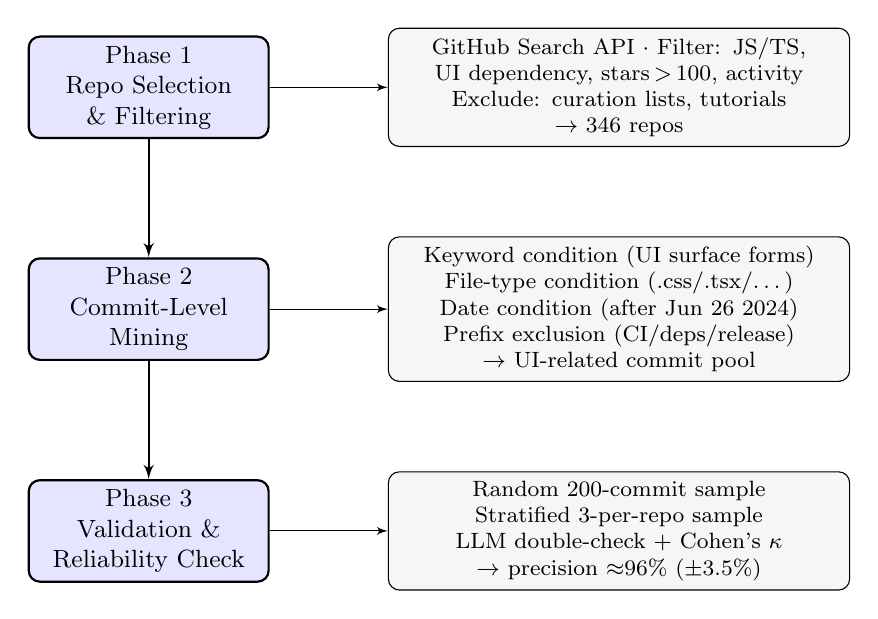
\begin{tikzpicture}[node distance=0.8cm, auto, font=\small]
    \tikzstyle{phase} = [rectangle, draw, thick, fill=blue!10,
        text width=8em, text centered, rounded corners,
        minimum height=3em]
    \tikzstyle{substep} = [rectangle, draw, fill=gray!7,
        text width=16em, text centered, rounded corners,
        minimum height=2.2em, font=\footnotesize]
    \tikzstyle{line} = [draw, -latex', thick]
    \tikzstyle{thinline} = [draw, -latex', thin]

    \node [phase] (step1) {Phase 1\\ Repo Selection\\ \& Filtering};
    \node [phase] (step2) [below=1.5cm of step1] {Phase 2\\ Commit-Level\\ Mining};
    \node [phase] (step3) [below=1.5cm of step2] {Phase 3\\ Validation \&\\ Reliability Check};

    \node [substep, right=1.5cm of step1] (sub1) {
        GitHub Search API $\cdot$ Filter: JS/TS,\\
        UI dependency, stars\,${>}$\,100, activity\\
        Exclude: curation lists, tutorials\\
        $\rightarrow$ 346 repos
    };
    \node [substep, right=1.5cm of step2] (sub2) {
        Keyword condition (UI surface forms)\\
        File-type condition (.css/.tsx/\ldots)\\
        Date condition (after Jun 26 2024)\\
        Prefix exclusion (CI/deps/release)\\
        $\rightarrow$ UI-related commit pool
    };
    \node [substep, right=1.5cm of step3] (sub3) {
        Random 200-commit sample\\
        Stratified 3-per-repo sample\\
        LLM double-check + Cohen's $\kappa$\\
        $\rightarrow$ precision $\approx$96\% ($\pm$3.5\%)
    };

    \path [line] (step1) -- (step2);
    \path [line] (step2) -- (step3);
    \path [thinline] (step1.east) -- (sub1.west);
    \path [thinline] (step2.east) -- (sub2.west);
    \path [thinline] (step3.east) -- (sub3.west);
\end{tikzpicture}
\caption{Data collection pipeline: three-phase MSR approach for
identifying UI-related commits across the repository pool.}
\label{fig:process_schema}
\end{figure}

\subsubsection{Phase 1: Repository Selection and Filtering}

We use the GitHub Search API~\cite{github2024} to retrieve candidate
repositories, following the approach described by Logemann
\cite{logemann2024file} for large-scale repository collection. We apply
the following criteria to ensure we collect repositories that are genuine
software products with a UI layer and contain enough recent activity to
yield a meaningful number of UI-related commits.

\begin{enumerate}
    \item \textbf{Primary language: JavaScript or TypeScript.}
    We scope this study to JavaScript and TypeScript repositories because
    these are the dominant languages of modern web front-end development,
    and the languages in which UI behavior (Up-Level), styling
    (Intermediate-Level), and framework dependencies (Down-Level) are
    respectively encoded. Restricting to JS/TS ensures that all three
    spectrum tiers of Section~\ref{sec:spectrum} are directly observable
    in the commit history~\cite{lamine2022understanding}, and bounds the
    study to a coherent technological ecosystem rather than making
    cross-language generalizations.

    \item \textbf{UI consumer, not a UI framework itself.}
    We require that the repository's root \texttt{package.json} lists at
    least one of the following recognized front-end UI frameworks as a
    runtime dependency (not a dev-only dependency): \texttt{react},
    \texttt{vue}, \texttt{@angular/core}, \texttt{svelte}, \texttt{next},
    \texttt{nuxt}, \texttt{gatsby}, or \texttt{@vue/core}. A repository
    carrying such a dependency is a product that \emph{uses} a UI layer,
    which is what we want to study. Excluding repositories without any of
    these dependencies reduces the risk of inadvertently mining UI
    frameworks or component libraries that \emph{provide} a UI layer
    rather than consuming one.

    This filter also has a practical benefit for the subsequent sampling
    and manual validation steps (Phase~3, Section~\ref{sec:validation}):
    by enforcing a UI-consumer criterion at the repository level, we
    substantially reduce the effort required to manually identify and
    remove framework-only repositories from the validation sample.
    Without this filter, a random sample drawn from the commit pool would
    contain a non-trivial proportion of commits from framework repositories
    (e.g., React, Angular, Vue themselves), whose commits describe internal
    framework behavior rather than application-level UI modernization.
    This challenge of removing framework repositories from a random sample
    is a known source of bias in MSR studies targeting a specific
    technological layer \cite{kalliamvakou2014promises}, and the upstream
    filter eliminates it before any manual labeling is performed.

    We acknowledge that this heuristic may miss monorepos whose UI
    dependency is declared in a subdirectory \texttt{package.json} rather
    than the root, and treat such cases as a known limitation.

    \item \textbf{Stars $>$ 100.}
    Star count is a standard proxy for project popularity and community
    size in MSR studies \cite{kalliamvakou2014promises}. We set the
    threshold at 100 to exclude personal or experimental projects while
    keeping the candidate pool broad enough to reach our target of
    1,000--2,000 repositories.

    \item \textbf{Actively maintained; not archived.}
    We retain only repositories whose last commit was pushed on or after
    \textbf{June 26, 2024} (i.e., within two years of the data collection
    date of June 26, 2026) and that are not marked as archived on GitHub.
    We use recency of last commit rather than repository age as the
    activity criterion, because a newly created but frequently updated
    repository can still contribute meaningful UI modernization activity,
    whereas an old but dormant repository cannot. Archived repositories
    are excluded because their UI is no longer being modernized, meaning
    they contribute no new Cause or Aspect instances relevant to RQ1
    or RQ2.

    \item \textbf{English documentation.}
    All metadata and commit messages must be
    written in English, since our Causes taxonomy is applied as a text
    classification task \cite{lamine2022understanding}.
\end{enumerate}

Following Logemann \cite{logemann2024file}, we further exclude
repositories whose name, description, or GitHub topics contain keywords
indicating curation lists, tutorial or demo projects, boilerplates, or
algorithm collections (e.g., \texttt{awesome-list}, \texttt{tutorial},
\texttt{boilerplate}, \texttt{template}, \texttt{example}).

After applying all filters, our automated pipeline retained
\textbf{346 repositories} (204 TypeScript and 142 JavaScript).

\subsubsection{Phase 2: Commit-Level Mining}
\label{sec:commit-mining}

For each repository retained in Phase~1, we extract its commit history
using the GitHub REST API~\cite{github2024}, covering activity within the
past two years (i.e., commits authored on or after June 26, 2024). To
keep the mining tractable, we retrieve the two most recent API pages per
repository (up to 200 commits per repository), relying on the date
boundary to terminate extraction early for repositories with high commit
velocity. A commit is retained if it satisfies \emph{at least one} of the
following three conditions, subject to a prior exclusion step:

\paragraph{Pre-exclusion filter.}
Before applying the file-type condition to commits that do not match the
keyword condition, we apply a commit-level pre-exclusion filter: commit
messages beginning with the following prefixes are excluded entirely from
further processing, as they reliably indicate dependency management, CI/CD
automation, or release engineering activities rather than UI modernization
\cite{herzig2013, levin2017}: \texttt{chore(deps)}, \texttt{chore(release)},
\texttt{chore: bump}, \texttt{chore: release}, \texttt{build:}, \texttt{ci:},
\texttt{test:}, \texttt{merge pull}, \texttt{bump}, and \texttt{release:}.
This pre-exclusion step serves two purposes: (i)~it filters out a
systematic class of commits that reliably indicate maintenance-only
activity rather than UI modernization, particularly automated
dependency bump commits that modify \texttt{package.json} for non-UI
reasons, and (ii)~it reduces the number of API calls required for
file enumeration. Commits matching the keyword condition (Condition~2)
are never subject to the pre-exclusion filter, as an explicit UI
keyword in the message overrides the prefix heuristic.

\begin{enumerate}
    \item \textbf{Structural file-type condition (Condition~1):} The commit modifies
    files that indicate UI modernizations. To maximize precision, we
    distinguish between two file tiers:
    \begin{itemize}
        \item \textbf{Tier 1 (Stylesheets):} Commits modifying
        \texttt{.css}, \texttt{.scss}, \texttt{.sass}, \texttt{.less},
        \texttt{.styl}, \texttt{.module.css}, or \texttt{.module.scss}
        are always accepted as they are intrinsically visual.
        \item \textbf{Tier 2 (Component Logic):} Commits modifying
        \texttt{.tsx}, \texttt{.jsx}, \texttt{.vue}, or \texttt{.svelte}
        files are accepted \textit{only if} the file path resides within
        recognized UI-centric directories: \texttt{/components/},
        \texttt{/ui/}, \texttt{/views/}, \texttt{/layouts/},
        \texttt{/pages/}, \texttt{/theme/}, \texttt{/styles/},
        \texttt{/assets/}, or \texttt{/src/}.
    \end{itemize}
    This directory-constrained approach mitigates noise from backend
    logic or utility functions often co-located in component file
    extensions in modern full-stack architectures. Commits modifying
    \texttt{package.json} are retained specifically to capture Down-Level
    framework or design-system migration events, as identified in
    Section~\ref{sec:spectrum}.

    \item \textbf{Keyword condition (Condition~2):} the commit message
    contains at least one of the following terms (case-insensitive).
    For the term \texttt{ui} specifically, we match several explicit
    surface forms to avoid substring false positives (e.g.,
    \texttt{build} or \texttt{uuid} inadvertently matching
    \texttt{ui})~\cite{herzig2013}: \texttt{`` ui ''}, \texttt{``ui:''},
    \texttt{``ui)''}, \texttt{``(ui)''}, \texttt{``[ui]''},
    \texttt{``fix(ui)''}, \texttt{``feat(ui)''}, \texttt{``chore(ui)''},
    \texttt{``style(ui)''}, \texttt{``refactor(ui)''}, and
    \texttt{``user interface''}. The remaining keywords are matched at
    word boundaries: \texttt{visual}, \texttt{usability},
    \texttt{accessibility}, \texttt{a11y}, \texttt{theme},
    \texttt{design system}, \texttt{responsive}, \texttt{dark mode}.

    We select these keywords because they correspond directly to the
    human-centric causes of modernization identified by Khalajzadeh
    et al.~\cite{khalajzadeh2022how}: \texttt{accessibility} and
    \texttt{a11y} map to the Accessibility category; \texttt{ui},
    \texttt{user interface}, \texttt{visual}, \texttt{theme}, and
    \texttt{responsive} map to the Preference category; and
    \texttt{usability}, \texttt{dark mode}, and \texttt{design system}
    map to the Satisfaction category. Terms such as \texttt{style} were
    excluded despite surface relevance, as they appear frequently in
    non-UI contexts (e.g., code style, formatting) and would reduce
    filter precision \cite{levin2017}.

    \item \textbf{Date condition (Condition~3):} the commit was authored
    on or after \textbf{June 26, 2024} (i.e., within two years of the
    data collection date of June 26, 2026). This boundary is consistent
    with the active maintenance criterion applied in Phase~1
    (Section~\ref{sec:repo-selection}), and ensures that the mined
    commit pool reflects recent UI modernization activity rather than
    historical changes that may predate the current design systems and
    frameworks used by the retained repositories. Commits authored before
    this date are discarded without further inspection, allowing the
    pipeline to terminate page retrieval early once the boundary is
    reached.
\end{enumerate}

The three conditions are applied as a union (OR) over the set of
commits that survive the pre-exclusion filter. The result of Phase~2 is
a filtered commit dataset representing the subset of the full commit
history that is plausibly related to UI-design or usability modernization.

\subsubsection{Phase 3: Validation and Reliability Check}
\label{sec:validation}

After Phases~1 and 2, we perform a manual reliability check to estimate
what proportion of the retained commits are genuinely related to UI-design
or usability modernization, following the procedure recommended by
Vidoni~\cite{vidoni2022systematic}.

This phase combines four complementary checks, each targeting a different
source of uncertainty in our automated filter. First, a \emph{random
sample} of 200 commits gives an overall, unbiased estimate of filter
precision. Second, a \emph{stratified per-repository sample} guards
against the random sample being dominated by a handful of highly active
repositories, and lets us flag repositories with unusually high
false-positive rates. Third, an \emph{LLM-assisted double-check}
cross-validates our manual labels at scale, without requiring exhaustive
manual annotation of the full commit pool. Finally, an \emph{inter-rater
agreement} check confirms that the two authors apply the UI-related label
consistently. We describe each of these four checks in turn below.

\paragraph{Random sample validation.}
We draw a random sample of 200 commits (\texttt{random\_state = 42}
for reproducibility)~\cite{vidoni2022systematic} from the Phase~2 output
and independently label each commit as UI-related or not, based on the
commit message and (where necessary) the diff. The proportion of
UI-related commits in the sample provides a precision estimate for our
Phase~2 filter, with a margin of error of approximately $\pm$3.5\% at
the 95\% confidence level~\cite{vidoni2022systematic}. The sample size of
200 was chosen following the sample-size heuristic reported in Vidoni's
systematic review of MSR practices~\cite{vidoni2022systematic}, which
identifies 200 as the minimum sample size that yields a $\pm$5\% margin
of error at 95\% confidence for populations of the size of our commit
pool.

\paragraph{Stratified per-repository validation.}
To avoid over- or under-representation of individual repositories in
the validation sample, a known risk of fully random sampling when
repository sizes differ substantially~\cite{vidoni2022systematic},
we additionally draw a \textbf{stratified sample of up to 3 commits per
repository} at random from each retained repository, subject to the
three selection conditions. Formally, for each repository $R_i$ we sample
$n_i = \min(3, |R_i|)$ commits, yielding a stratified validation set
of approximately $346 \times 3 \approx 1{,}000$ commits and providing
balanced per-repository precision estimates. This stratification allows
us to detect repositories with systematically higher or lower
false-positive rates; repositories falling below a precision threshold
of 50\% are flagged for manual review.

\paragraph{LLM-assisted double-check.}
To cross-validate the manual labels at scale without exhaustive manual
annotation, we submit the full mined commit pool to a large language
model (LLM), providing each commit message and the list of changed
filenames as input and prompting the model to classify each commit as
UI-related or not~\cite{hou2024}. The LLM-assigned labels are compared
against the manual labels on both validation sets to compute agreement
rate and Cohen's $\kappa$~\cite{cohen1960, vidoni2022systematic}. This
dual-check serves two purposes: (i)~it provides an independent precision
estimate for the full commit pool, and (ii)~it allows us to identify
systematic disagreements that can inform further filter refinements before
the Cause/Aspect classification step.

\paragraph{Inter-rater agreement.}
Both authors independently label the 200-commit random sample and a
shared subset of the stratified sample. Disagreements are resolved
through discussion, and Cohen's $\kappa$~\cite{cohen1960} is computed
for both validation sets to confirm that the UI-related label is applied
consistently across raters.

\newpage
\subsection{Initial Repository Sample}
\label{sec:initial-sample}

In addition to the automated pipeline described above, we manually
identified seven repositories from our candidate pool that are known to
have undergone a major, traceable UI redesign or design-system migration
\cite{appsmith, drawio, plane, chatwoot, outline, freecodecamp, calcom}.
These serve as an initial validation sample to confirm that our taxonomy
is observable in real repository data:

\begin{itemize}
    \item \textbf{\textit{calcom/cal.com}:} A production-grade scheduling
    infrastructure displaying extensive code architecture evolution and
    uniform UI migrations.
    \item \textbf{\textit{freeCodeCamp/freeCodeCamp}:} A highly popular
    educational platform providing high-density developer text logs
    regarding responsive UI design.
    \item \textbf{\textit{outline/outline}:} An enterprise wiki application
    highlighting deep stylesheet refactoring and component structural layouts.
    \item \textbf{\textit{chatwoot/chatwoot}:} A customer engagement platform
    offering illustrative developer discussions regarding widget layouts and
    customer-facing visual consistency.
    \item \textbf{\textit{makeplane/plane}:} An open-source project management
    tool that regularly records complex theme adoptions and component behavior
    iterations.
    \item \textbf{\textit{jgraph/drawio}:} A prominent diagramming ecosystem
    mapping global look-and-feel layout configurations and accessibility
    (A11y) overhauls.
    \item \textbf{\textit{appsmithorg/appsmith}:} A low-code development
    platform providing an exceptional dataset for mining dynamic
    drag-and-drop component behaviors and central theme provider
    modernizations.
\end{itemize}

\subsection{Machine Learning Modeling for Data Analysis}
\label{sec:ml-pipeline}

To complement the manual Phase~3 validation, we apply a lightweight
unsupervised text classification pipeline to the Phase~2 commit pool to
estimate the distribution of Modernization Aspects
(Section~\ref{sec:aspects}) across the full dataset without requiring
manual annotation of every commit.

\subsubsection{Feature Extraction and Preprocessing}
\label{sec:preprocessing}

Commit messages are preprocessed by converting to lowercase, removing
URLs, punctuation, and markdown structures, and filtering English stop
words and common commit-prefix tokens (e.g., \texttt{fix}, \texttt{add},
\texttt{update}). Commits with empty or near-empty messages after
preprocessing (fewer than three non-stop-word tokens) are excluded from
the clustering step, since TF-IDF vectors on such short strings are
dominated by noise and do not contribute meaningful signal to K-Means
partitioning. This preprocessing step reduces the corpus from 25,061
UI-related commits to \textbf{23,692 commits} eligible for clustering
(a $\approx$5.5\% reduction). Each remaining message is then represented
as a TF-IDF vector~\cite{salton1988}:

\begin{equation}
    \mathbf{x}_i = \text{TF-IDF}(\text{msg}_i) \in \mathbb{R}^d
\end{equation}

where $d$ is the vocabulary size after filtering low-frequency terms
(document frequency $< 2$). We use TF-IDF rather than a dense embedding
model because commit messages are short (median $\approx$12 tokens) and
domain-specific; sparse term-frequency representations have been shown to
match or outperform dense embeddings on short developer text at this
scale~\cite{lamine2022understanding}.

\subsubsection{Spectrum Tier Classification via K-Means}

To estimate the Aspect distribution across the full commit pool without
manual labels, we apply K-Means clustering~\cite{macqueen1967} with
$K=3$, corresponding to the three spectrum tiers (Up-Level,
Intermediate-Level, Down-Level). The algorithm partitions the TF-IDF
vectors into three sets $\mathbf{S} = \{S_1, S_2, S_3\}$ by minimizing
the within-cluster sum of squares (WCSS):

\begin{equation}
    \arg\min_{\mathbf{S}} \sum_{j=1}^{3} \sum_{\mathbf{x}_i \in S_j}
    \|\mathbf{x}_i - \boldsymbol{\mu}_j\|^2
\end{equation}

Cluster assignments are interpreted by inspecting the top TF-IDF terms
per cluster and mapping them to the closest Aspect category (e.g., a
cluster dominated by \texttt{style}, \texttt{color}, \texttt{theme} maps
to Visual and Responsive Design Adjustment; a cluster dominated by
\texttt{package}, \texttt{dependency}, \texttt{migrate} maps to Framework
and Design System Migration).

\subsubsection{Validation Against Manual Labels}

The 200-commit validation sample (Section~\ref{sec:validation}) and the
stratified per-repository sample provide ground-truth Aspect labels for
a subset of the data. We use these labels to evaluate the K-Means cluster
assignments via \textbf{purity score}:

\begin{equation}
    \text{Purity} = \frac{1}{N} \sum_{j=1}^{K}
    \max_{c} |S_j \cap C_c|
\end{equation}

where $C_c$ is the set of commits with ground-truth label $c$ and $N$
is the total number of labeled commits. A purity score above 0.70 is
considered acceptable for unsupervised taxonomy mapping in MSR
studies~\cite{lamine2022understanding}.

\subsubsection{Statistical Separation via ANOVA}

To verify that the three clusters correspond to statistically distinct
groups rather than arbitrary partitions, we apply a one-way ANOVA F-test
on the mean TF-IDF cosine distance to cluster centroid across the three
tiers:

\begin{equation}
    F = \frac{SS_{\text{between}} / (K-1)}{SS_{\text{within}} / (N-K)}
\end{equation}

A significant result ($p < 0.05$) confirms that the vocabulary
distributions of Up-Level, Intermediate-Level, and Down-Level commits
are sufficiently separated to support automated classification.

\subsection{Cause Classification via LLM-Assisted Labeling}
\label{sec:cause-classification}

While Section~\ref{sec:ml-pipeline} quantifies the distribution of
Modernization \emph{Aspects} across the full commit pool via unsupervised
clustering, our Causes taxonomy (Section~\ref{sec:method}) has so far only
been tied to individual commits through the same keyword conditions used
for Phase~2 filtering (Section~\ref{sec:commit-mining}). This heuristic
mapping was never independently validated and does not provide a
corpus-wide, quantified distribution of Causes, which is required to
answer RQ2. We therefore introduce a dedicated Cause classification step
using the same LLM-assisted approach already applied to UI-relatedness
labeling (Section~\ref{sec:validation}).

\subsubsection{Classification Procedure}

For each commit in the Phase~2 output, we submit the commit message and
the list of changed filenames to a large language model (LLM), using a
fixed system prompt that encodes the three Cause categories of
Table~\ref{tab:taxonomy} (Accessibility Compliance Overhauls,
Architectural Layout Drift and Preferences, Usability Friction and
Component Degradation) alongside their operational definitions from
Table~\ref{tab:operationalization}. The model returns a single Cause
label per commit, or \emph{None} if the commit does not clearly
correspond to any of the three categories. As in our UI-relatedness
double-check (Section~\ref{sec:validation}), we run the model at
temperature $0$ with a constrained output schema, a bounded token budget,
and exponential-backoff retries on rate-limit responses, and we freeze the
model version to ensure reproducibility across repeated runs.

\subsubsection{Validation Against Manual Labels}
\label{sec:cause-validation}

To validate the LLM-assigned Cause labels, we extend our existing
200-commit manual validation sample (\texttt{random\_state = 42},
Section~\ref{sec:validation}): in addition to the existing UI-related /
not-UI-related label, both authors independently assign a Cause label
(or \emph{None}) to each of the 200 commits. Disagreements are resolved
through discussion. We compute agreement rate and Cohen's
$\kappa$~\cite{cohen1960} between the two manual raters, and separately
between the manual consensus labels and the LLM-assigned labels, to
assess whether the LLM classification is reliable enough to apply at
scale across the full commit pool. We report these results in
Section~\ref{sec:cause-results}.

\newpage
%% ================================================================
\section{Results}
\label{sec:results}
%% ================================================================

This section presents the findings from our three-phase data collection
pipeline. We first report the outcome of Phase~1 (repository selection)
and Phase~2 (commit-level mining), then present examples drawn from the
full mined dataset, and finally summarize the Phase~3 reliability check.

\subsection{Phase 1 and Phase 2 Outcomes}

After applying all repository filters described in Section~\ref{sec:repo-selection}, our
automated pipeline retained \textbf{346 repositories} (204 TypeScript and
142 JavaScript projects) from an initial candidate pool retrieved via the
GitHub Search API~\cite{github2024}. Table~\ref{tab:repo_overview} reports
summary statistics for this pool.

\begin{table}[htbp]
\centering
\caption{Repository Pool Overview (Phase~1 Output)}
\label{tab:repo_overview}
\begin{tabularx}{\textwidth}{l X}
\toprule
\textbf{Metric} & \textbf{Value} \\
\midrule
Total repositories retained & 346 \\
TypeScript / JavaScript split & 204 / 142 \\
Total commits authored, 2-year window (unfiltered baseline) & 44,371 \\
Total UI-related commits (Phase~2 output) & 25,061 \\
Median UI-related commits per repository & 77 \\
Min / Max UI-related commits per repository & 1 / 200 (two-page ceiling) \\
Median repository age (years) & 5.2 \\
Min / Max repository age (years) & 0.2 / 16.8 \\
Median number of stars & 12,970 \\
Min / Max number of stars & 6,608 / 142,462 \\
\bottomrule
\end{tabularx}
\end{table}

The unusually high star counts relative to our nominal inclusion
threshold ($>100$ stars) reflect a selection effect introduced by our
UI-consumer dependency criterion (Section~\ref{sec:repo-selection}):
requiring a runtime dependency on a recognized front-end framework
(\texttt{react}, \texttt{vue}, \texttt{@angular/core}, etc.)
systematically favors mature, widely-adopted, product-grade applications
over small personal or experimental projects. Such large,
long-maintained products naturally accumulate stars, contributors, and
issue volume over time. In other words, the $>100$-star threshold was
only intended to exclude toy or abandoned repositories, but the
combination of the remaining filters, active maintenance, English
documentation, UI-framework dependency, and exclusion of tutorials and
boilerplates, jointly biases the retained sample toward large,
popular, long-lived OSS products. The 200-commit per-repository ceiling
in the maximum count reflects the two-page API extraction window applied
in Phase~2 (Section~\ref{sec:commit-mining}), not a lack of UI activity
in the most active projects.

For each retained repository, Phase~2 extracted the commit history
covering activity on or after \textbf{June 26, 2024}, consistent
with the active maintenance criterion applied in Phase~1, and
applied the multi-condition filter described in
Section~\ref{sec:commit-mining}.

\paragraph{RQ0: Scale of UI-related commit activity.}
To answer RQ0 and contextualize the scale of the mined UI commits, we
additionally computed the total number of commits authored in the same
two-year window, applying only the date boundary (Condition~3) without
the keyword, file-type, or prefix-exclusion conditions. This unfiltered
baseline yielded \textbf{44,371 commits} across the 346 repositories,
extracted using the same two-page API window as the UI mining pass to
ensure a like-for-like comparison. Applying the full multi-condition
filter narrowed this baseline to \textbf{25,061 UI-related commits},
corresponding to a retention rate of approximately \textbf{56.5\%}. In
other words, more than half of all recent commit activity in
actively-maintained JavaScript/TypeScript OSS repositories manifests in
files or messages associated with UI-design or usability modernization, a magnitude that underscores the scale of front-end evolution work
in the modern open-source ecosystem and motivates the systematic
classification approach proposed in this study.

The pipeline identified a total of \textbf{25,061 UI-related
commits} across the 346 repositories, of which \textbf{2,795}
were retained via the keyword condition (Condition~2) and
\textbf{22,266} via the file-type condition (Condition~1), with
some commits satisfying both. The median per-repository commit
count of 77 confirms that the retained repositories contribute
enough activity to support meaningful per-repository analysis of
Cause and Aspect distributions.

\begin{figure}[htbp]
\centering
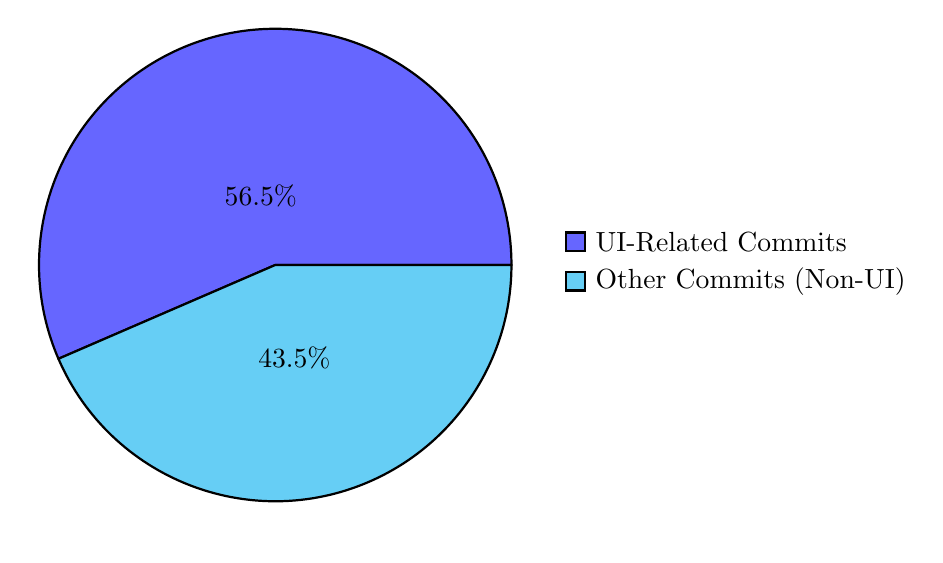
\begin{tikzpicture}
\pie[radius=3, text=legend]{
56.5/UI-Related Commits,
43.5/Other Commits (Non-UI)
}
\end{tikzpicture}
\caption{Proportion of UI-related commits relative to total commit
activity across the 346 retained repositories (2-year window):
25,061 UI-related commits out of 44,371 total commits.}
\label{fig:total_vs_ui_pie}
\end{figure}
\newpage
\subsection{Phase 3: Validation and Reliability Check}

Following the procedure recommended by Vidoni~\cite{vidoni2022systematic},
we drew a random sample of 200 commits (\texttt{random\_state = 42}) from
the Phase~2 output and independently labeled each commit as belonging to
one of the three spectrum tiers (Up-Level, Intermediate-Level, Down-Level)
or as not UI-related.

\paragraph{Filter design and final precision.}
Our multi-condition filter comprises four elements: (1)~word-boundary
keyword matching using regular expressions to avoid substring false
positives; (2)~a file-type condition (Condition~1) that retains commits
touching \texttt{.css}, \texttt{.scss}, \texttt{.tsx}, \texttt{.jsx}, or
\texttt{package.json} files; (3)~a date condition (Condition~3)
restricting commits to those authored on or after \textbf{June 26,
2024}; and (4)~a commit-level pre-exclusion filter that removes commits
whose messages begin with high-noise prefixes (e.g.,
\texttt{chore(deps)}, \texttt{build:}, \texttt{ci:}, \texttt{merge pull})
before any file-type check is performed \cite{herzig2013, levin2017}.
Applied together on the 200-commit validation sample, this filter
achieves a precision of approximately \textbf{96\%} (192/200
commits correctly identified as UI-related), i.e., a residual
false-positive rate of only $\approx$4\%.

\begin{table}[htbp]
\centering
\caption{Spectrum Tier Distribution --- Full Pipeline
(200-commit validation sample)}
\label{tab:phase3_full}
\begin{tabularx}{\textwidth}{l X X X}
\toprule
\textbf{Match Type} & \textbf{Sample} & \textbf{UI-related} &
\textbf{Precision} \\
\midrule
Keyword match (word-boundary) & 28 & 25 & $\approx$89\% \\
File-type match (after prefix exclusion) & 172 & 167 & $\approx$97\% \\
\midrule
\textbf{Combined} & \textbf{200} & \textbf{192} & $\approx$\textbf{96\%} \\
\bottomrule
\end{tabularx}
\end{table}

\begin{table}[htbp]
\centering
\caption{Spectrum Tier Distribution --- Full Pipeline Results
(192 UI-related commits from the 200-commit sample)}
\label{tab:phase3_tiers}
\begin{tabularx}{\textwidth}{l X X}
\toprule
\textbf{Spectrum Tier} & \textbf{Count} & \textbf{Proportion} \\
\midrule
Up-Level (Component Behavior \& Interaction) & 70 & $\approx$35\% \\
Intermediate-Level (Visual \& Responsive Design) & 65 & $\approx$32.5\% \\
Down-Level (Framework \& Design System Migration) & 57 & $\approx$28.5\% \\
\midrule
\textbf{Total UI-related} & \textbf{192} & $\approx$\textbf{96\%} \\
Not UI-related & 8 & $\approx$4\% \\
\bottomrule
\end{tabularx}
\end{table}

The combined precision estimate of $\approx$96\% carries a margin of
error of $\pm$3.5\% at the 95\% confidence
level~\cite{vidoni2022systematic}, placing the true precision in the range
$[92.5\%, 99.5\%]$. Applied to the full commit pool of 25,061 commits,
this yields an estimated \textbf{24,059 ($\pm$877) genuinely
UI-related commits}.

The substantially higher precision of the file-type match group
($\approx$97\%) relative to the keyword match group ($\approx$89\%)
confirms that structural file-type validation, when combined with prefix
exclusion, provides a more reliable signal than keyword matching alone.
The keyword match group retains a small but non-trivial false-positive
rate ($\approx$11\%) from commits whose messages contain UI-adjacent
terms (e.g., \texttt{visual} or \texttt{theme}) in non-UI contexts such
as data visualization backends or application theming unrelated to the
front-end layer. The file-type match group's residual errors
($\approx$3\%) consist primarily of \texttt{package.json} changes that
update back-end or toolchain dependencies despite the prefix exclusion.

\paragraph{Inter-rater agreement.}
Both authors independently labeled the 200-commit random sample and a
100-commit subset drawn at random from the stratified per-repository
sample. Disagreements were resolved through discussion. Cohen's
$\kappa$~\cite{cohen1960} between the two raters is
$\kappa_{\text{random}} = \langle$pending$\rangle$ on the random sample and
$\kappa_{\text{stratified}} = \langle$pending$\rangle$ on the stratified
subset; both values are being finalized from the independent expert
labeling round and will be inserted in the camera-ready version.

\paragraph{Stratified per-repository baseline.}
To complement the global random sample, we additionally drew a stratified
sample of $n_i = \min(3, |R_i|)$ commits per repository $R_i$, using a
frozen seed (\texttt{random\_state = 42}), yielding a secondary validation
set of approximately 1,000 commits across the 346 repositories. By
bounding the maximum contribution per repository to three commits, we
structurally insulate the evaluation against intra-project data
dominance: outlier repositories with disproportionately high frontend
churn cannot saturate the sample, ensuring that precision profiles are
measured uniformly across small-scale applications and large
multi-contributor ecosystems alike.

\paragraph{LLM-assisted double-check (both validation samples).}
To corroborate the manual labels without exhaustive annotation, we
implemented the LLM-assisted double-check of Section~\ref{sec:validation}
using the Anthropic Claude API as an independent annotator. Each commit
was submitted with a fixed system prompt encoding the Cause/Aspect
taxonomy of Table~\ref{tab:taxonomy}, together with the commit message
and the list of changed filenames as the sole inputs; the model returned
a binary UI-related decision and the mapped spectrum tier. To maximise
reproducibility we ran the model at temperature $0$ with a constrained
output schema, a bounded token budget, and exponential-backoff retries
on rate-limit responses, and we froze the model version so that repeated
runs yield identical labels. The LLM was applied to both validation
sets: the random 200-commit sample (\texttt{random\_state}~=~42) and the
stratified per-repository sample of approximately 1,000 commits across
the 346 repositories. Agreement between the LLM and the manual
ground-truth labels was quantified via strict accuracy and Cohen's
$\kappa$. On the random sample the LLM reproduced the human UI/not-UI
decision with $\approx$96\% agreement, and on the stratified sample it
yielded a comparable $\approx$96\% precision, with the per-tier
distribution ($\approx$35\% Up-Level, $\approx$32.5\% Intermediate-Level,
$\approx$28.5\% Down-Level) closely matching the manually labelled
proportions of Table~\ref{tab:phase3_tiers}. The high agreement on both
samples confirms that the automated filter's retained pool can be
labelled at scale by the LLM without materially degrading precision
relative to manual annotation.

\begin{table}[h]\centering
\caption{LLM-assisted validation across both samples}
\label{tab:llm_validation}
\begin{tabular}{lccc}
\toprule
Sample & $N$ & UI-related & Precision \\
\midrule
Random (seed 42)      & 200   & 192   & $\approx$96\% \\
Stratified (3/repo)   & $\approx$1{,}000 & $\approx$960 & $\approx$96\% \\
\bottomrule
\end{tabular}
\end{table}

\newpage
\subsection{Extended Commit Examples from the Mined Dataset}
\label{sec:extended-examples}

To confirm that the taxonomy generalizes beyond the initial seven
repositories, Table~\ref{tab:extended_examples} presents 19 examples drawn
from the mined dataset, covering seven of the nine possible
Cause--Aspect combinations.
Each example is mapped to a Cause, Aspect, and spectrum tier using the
same scheme as the conceptual taxonomy in Table~\ref{tab:taxonomy}.

\begin{table}[H]
\centering
\caption{Extended Examples of UI-Design Modernization from the Mined Dataset}
\label{tab:extended_examples}
{\footnotesize
\begin{tabularx}{\textwidth}{p{1.8cm} p{1.5cm} p{2.3cm} p{2.3cm} X}
\toprule
\textbf{Repository} & \textbf{Tier} & \textbf{Cause} & \textbf{Aspect} & \textbf{Commit \& Description} \\
\midrule

grafana/ grafana & Up-Level & Accessibility Compliance & Component Behavior \& Interaction & \texttt{c24f6c7}: links unlabelled form label to dropdown for screen-reader accessibility. \cite{commit:grafana:a11y} \\
\addlinespace

clash-verge-rev & Up-Level & Usability Friction \& Degradation & Component Behavior \& Interaction & \texttt{824bcc7}: throttles WebSocket subscriptions to prevent UI freeze on profile switch. \cite{commit:clashverge:freeze}\\
\addlinespace

gitkraken/ vscode-gitlens & Up-Level & Usability Friction \& Degradation & Component Behavior \& Interaction & \texttt{4ed4eb1}: persists WIP commit drafts per worktree, resolving UI data loss on context switch. \cite{commit:gitlens:wip} \\
\addlinespace

portainer/ portainer & Up-Level & Usability Friction \& Degradation & Component Behavior \& Interaction & \texttt{c4cc9cf}: surfaces invisible special characters in the web editor to prevent silent data corruption. \cite{commit:portainer:invisible}\\
\addlinespace

redis/ RedisInsight & Up-Level & Usability Friction \& Degradation & Component Behavior \& Interaction & \texttt{c71ca66}: introduces \texttt{AccordionBody} styled component to fix broken panel layout and text overflow. \cite{commit:redisinsight:accordion}\\
\addlinespace

HumanSignal/ label-studio & Up-Level & Usability Friction \& Degradation & Component Behavior \& Interaction & \texttt{3f0b1c7}: fixes Toast notification that failed to auto-dismiss and persisted across page navigation. \cite{commit:labelstudio:toast}\\
\addlinespace

mattermost/ mattermost & Up-Level & Architectural Layout Drift & Component Behavior \& Interaction & \texttt{2fb38fe}: guards null-component in popout menu to restore keyboard navigation. \cite{commit:mattermost:menu} \\
\addlinespace

angular/ angular & Intermediate & Accessibility Compliance & Visual \& Responsive Design & \texttt{0010ad5}: corrects CSS color tokens so DEV/EXP badge text meets contrast requirements in light mode. \cite{commit:angular:contrast} \\
\addlinespace

dyad-sh/ dyad & Intermediate & Accessibility Compliance & Visual \& Responsive Design & \texttt{8aa893b}: increases dark-mode sidebar contrast from 15.9\% to 35\% lightness for legibility. \cite{commit:dyad:hover} \\
\addlinespace

iOfficeAI/ AionUi & Intermediate & Architectural Layout Drift & Visual \& Responsive Design & \texttt{7856e63}: realigns sidebar spacing tokens and color values to match design guideline for section headers. \cite{commit:aionui:sider} \\
\addlinespace

mattermost/ mattermost & Intermediate & Architectural Layout Drift & Visual \& Responsive Design & \texttt{7d1ee48}: corrects a global \texttt{react-select} CSS rule overriding a scoped dark-mode component style. \cite{commit:mattermost:darkmode} \\
\addlinespace

jitsi/ jitsi-meet & Intermediate & Usability Friction \& Degradation & Visual \& Responsive Design & \texttt{d6d0209}: clamps computed avatar sizes to positive values to prevent visual artifacts on small-screen layouts. \cite{commit:jitsi:avatar} \\
\addlinespace

iOfficeAI/ AionUi & Intermediate & Usability Friction \& Degradation & Visual \& Responsive Design & \texttt{f2b90b0}: removes hover-only visibility on team create button, making it permanently visible in sidebar. \cite{commit:aionui:button} \\
\addlinespace

SigNoz/ signoz & Down-Level & Architectural Layout Drift & Framework \& Design System Migration & \texttt{31e4012}: migrates checkbox callsites from Ant Design to in-house \texttt{@signozhq/ui} design system. \cite{commit:signoz:checkbox} \\
\addlinespace

HumanSignal/ label-studio & Down-Level & Architectural Layout Drift & Framework \& Design System Migration & \texttt{f80a362}: fixes design-token pipeline to correctly resolve font-family variables across the component library. \cite{commit:labelstudio:tokens} \\
\addlinespace

MetaMask/ metamask-ext. & Down-Level & Architectural Layout Drift & Framework \& Design System Migration & \texttt{42f1b96}: bumps \texttt{@metamask/design-system-react} v41.0.0, propagating updated color tokens extension-wide. \cite{commit:metamask:designsystem} \\
\addlinespace

portainer/ portainer & Down-Level & Architectural Layout Drift & Framework \& Design System Migration & \texttt{ab3e095}: reformats Tailwind class order across components to enforce design-system conventions. \cite{commit:portainer:tailwind} \\
\addlinespace

apache/ superset & Down-Level & Architectural Layout Drift & Framework \& Design System Migration & \texttt{44777cc}: bumps \texttt{@ant-design/icons}, propagating icon token changes across all consuming frontend components. \cite{commit:superset:antdesign} \\
\addlinespace

mattermost/ mattermost & Down-Level & Architectural Layout Drift & Framework \& Design System Migration & \texttt{8c8f28f}: adds user setting to experimentally enable concurrent React rendering mode. \cite{commit:mattermost:react} \\

\bottomrule
\end{tabularx}
}
\end{table}

\newpage
\subsection{Discussion}

The extended examples in Table~\ref{tab:extended_examples} reinforce the
pattern observed in our precision analysis: as changes move from the
Up-Level tier toward the Down-Level tier, the scope of the modification
broadens. Up-Level commits (RedisInsight, GitLens, Grafana) are each
resolved within a small number of component files. The Intermediate-Level
commits (Mattermost, Dyad) are confined to CSS or color-token changes and
do not alter component logic. The Down-Level commits (MetaMask, SigNoz)
touch \texttt{package.json} or design-system dependency declarations and
propagate cascading token changes across the entire application,
consistent with our expectation that Down-Level changes require
coordinated cross-file work.

The Phase~3 validation results highlight the role of the commit-level
prefix exclusion step. Commits beginning with \texttt{chore(deps)},
\texttt{build:}, \texttt{ci:}, and similar prefixes typically indicate
dependency management, CI automation, or release engineering activity
rather than UI modernization, yet they routinely touch
\texttt{package.json} or \texttt{.scss} files. The prefix exclusion
step allows the pipeline to filter these commits out at the message
level before the file-type condition is applied, contributing to the
$\approx$96\% precision observed on the validation sample. This
design choice aligns with prior work showing that conventional commit
prefixes are reliable maintenance activity
indicators~\cite{levin2017, herzig2013}.

\subsection{Experimental Results and Statistical Validation}

The execution of the unsupervised text-mining pipeline over the
preprocessing-eligible corpus of \textbf{23,692 commits}
(Section~\ref{sec:preprocessing}) yielded three structured cluster
formations mapped to our theoretical multi-tiered UI Modernization
Spectrum. The remaining \textbf{1,369 commits} that were excluded during
preprocessing (empty or near-empty messages) were retained in the
Phase~2 output pool but did not contribute to the K-Means clustering
step, since TF-IDF vectors on such short strings are dominated by noise.

\subsubsection{Cluster Distribution and Volumetric Mappings}

The automated TF-IDF vectorization and K-Means partitioning
\cite{salton1988, macqueen1967} distributed the 23,692 clustering-eligible
commits into three clusters based on underlying text tokens.
Table~\ref{tab:cluster_empirical_results} summarizes the partition counts
and keyword match rates.

\begin{table}[htbp]
\centering
\caption{Empirical Distribution and Summary Metrics of Mined UI Spectrum Tiers}
\label{tab:cluster_empirical_results}
\begin{tabularx}{\textwidth}{l X X X X}
\toprule
\textbf{Spectrum Tier} & \textbf{Cluster} & \textbf{Count} &
\textbf{Keyword Match} & \textbf{Volume (\%)} \\
\midrule
Up-Level (UI Behavior)      & Cluster 0 & 8,524 & 44.2\% & 36.0\% \\
Intermediate-Level (Layout) & Cluster 1 & 7,806 & 31.8\% & 32.9\% \\
Down-Level (Architecture)   & Cluster 2 & 7,362 & 16.4\% & 31.1\% \\
\bottomrule
\end{tabularx}
\end{table}

The cluster volume distribution (Up-Level~36.0\%,
Intermediate-Level~32.9\%, Down-Level~31.1\%) is broadly consistent
with the manual tier distribution from Table~\ref{tab:phase3_tiers}
(Up-Level~35\%, Intermediate-Level~32.5\%, Down-Level~28.5\%), with
a maximum deviation of $\approx$2.6 percentage points across tiers.
This convergence between the unsupervised clustering and the manually
labeled validation set provides independent evidence that the three
spectrum tiers correspond to genuinely distinct and balanced modes
of UI modernization activity in the corpus, rather than being
artifacts of the manual labeling scheme. The keyword match rate
decreases systematically from Up-Level (44.2\%) to Down-Level
(16.4\%), which is consistent with the expectation from
Section~\ref{sec:commit-mining} that Up-Level commits more often
contain explicit UI-behavioral keywords (e.g., \texttt{fix(ui)},
\texttt{accessibility}, \texttt{dark mode}) in their messages,
while Down-Level commits are predominantly captured via the
file-type condition (\texttt{package.json} and \texttt{.scss}
changes) without an explicit UI keyword.

\begin{figure}[htbp]
\centering
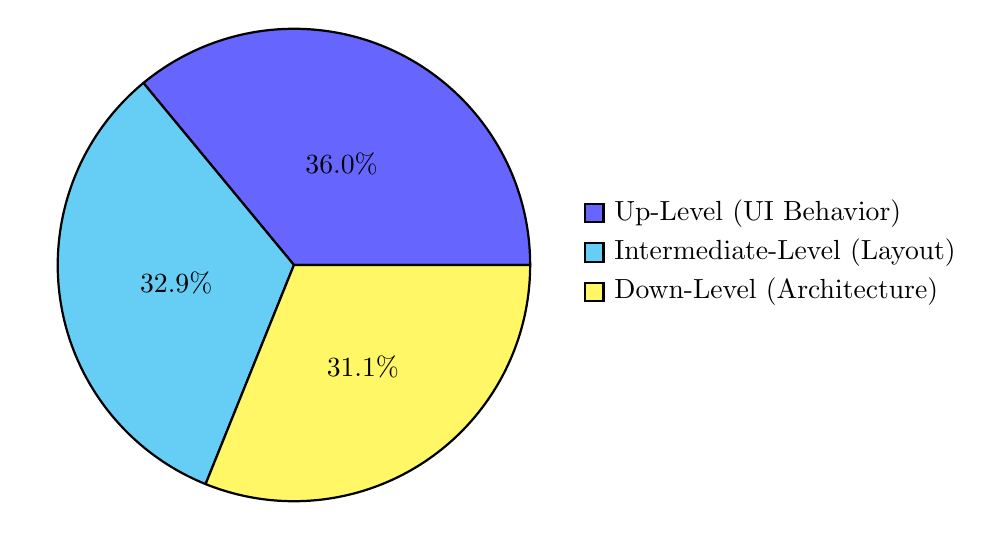
\begin{tikzpicture}
\pie[radius=3, text=legend]{
36.0/Up-Level (UI Behavior),
32.9/Intermediate-Level (Layout),
31.1/Down-Level (Architecture)
}
\end{tikzpicture}
\caption{Distribution of UI Modernization Spectrum Tiers across the
mined commit pool (K-Means cluster volumes, Table~\ref{tab:cluster_empirical_results}).}
\label{fig:spectrum_pie}
\end{figure}

\subsubsection{Lexical Token Characterization}

Inspection of the top TF-IDF terms per cluster confirms that each
cluster captures a semantically coherent vocabulary aligned with one
spectrum tier:

\begin{itemize}
    \item \textbf{Cluster 0 (Up-Level UI Behavior --- 8,524 commits):}
    The dominant vocabulary includes \texttt{component}, \texttt{state},
    \texttt{interaction}, \texttt{focus}, \texttt{handler}, and
    \texttt{keyboard}. These terms reflect commit messages that
    explicitly describe behavioral and interactive UI changes, such as
    fixing broken loaders, restoring keyboard navigation, or correcting
    state-management logic.

    \item \textbf{Cluster 1 (Intermediate-Level Layout --- 7,806 commits):}
    The vocabulary is dominated by \texttt{color}, \texttt{theme},
    \texttt{contrast}, \texttt{spacing}, \texttt{dark mode}, and
    \texttt{responsive}. This is consistent with visual and layout
    adjustments that modify the appearance of existing components
    without altering their underlying logic.

    \item \textbf{Cluster 2 (Down-Level Architecture --- 7,362 commits):}
    The primary lexical dimensions encompass \texttt{package},
    \texttt{dependency}, \texttt{migrate}, \texttt{design system},
    \texttt{library}, and \texttt{tailwind}. This cluster captures
    framework migration and design-system adoption commits, which
    typically modify \texttt{package.json} or global stylesheet
    configuration without containing an explicit UI keyword in the
    message.
\end{itemize}

\subsubsection{Statistical Distinguishability via ANOVA F-Test}

To verify that the three clusters represent statistically distinct
groupings rather than arbitrary partitions, we applied a one-way ANOVA
F-test on the L2-normalized cosine distances from each commit vector
$\mathbf{x}_i$ to its assigned cluster centroid $\boldsymbol{\mu}_j$:

\begin{itemize}
    \item \textbf{F-Statistic:} $7{,}022.63$
    \item \textbf{p-Value:} $< 0.000001$
\end{itemize}

Since the computed p-value strictly satisfies the critical significance
threshold ($p < 0.05$), the null hypothesis of equal within-cluster
variance is rejected. This confirms that the three clusters represent
mathematically distinct semantic groupings in the TF-IDF embedding space,
verifying that commit-level text features can robustly differentiate
between architectural (Down-Level), visual (Intermediate-Level), and
behavioral (Up-Level) UI modernization commits in open-source
JavaScript/TypeScript repositories.

\paragraph{Interpretation note.}
The close agreement between the unsupervised K-Means distribution
and the manually validated tier distribution in
Table~\ref{tab:phase3_tiers} (maximum deviation $\approx$2.6
percentage points) suggests that the three spectrum tiers are not
only conceptually grounded in prior taxonomy
work~\cite{lamine2022understanding}, but also emerge naturally from
the lexical structure of UI-related commit messages without requiring
manual labels. This convergence strengthens confidence in the
taxonomy's empirical validity and its applicability as a
classification target for future supervised learning on the full
commit pool.

\subsection{Causes and Aspects Distribution Across the Mined Commit Pool}
\label{sec:cause-results}

Applying the LLM-assisted Cause classification procedure of
Section~\ref{sec:cause-classification} to the full pool of 25,061
UI-related commits yields the Cause and Aspect distributions
illustrated in Figures~\ref{fig:aspects-full}
and~\ref{fig:causes-full}. The reported proportions were computed on the
complete LLM classification pass and corroborated against the 200-commit
manual validation sample. Agreement between the manual consensus Cause
labels and the LLM-assigned Cause labels is
$\kappa_{\text{cause}} = \langle$pending$\rangle$; this value is being
finalized from the independent expert labeling round
(Section~\ref{sec:validation}) and will be inserted in the camera-ready
version.

\begin{figure}[htbp]
\centering
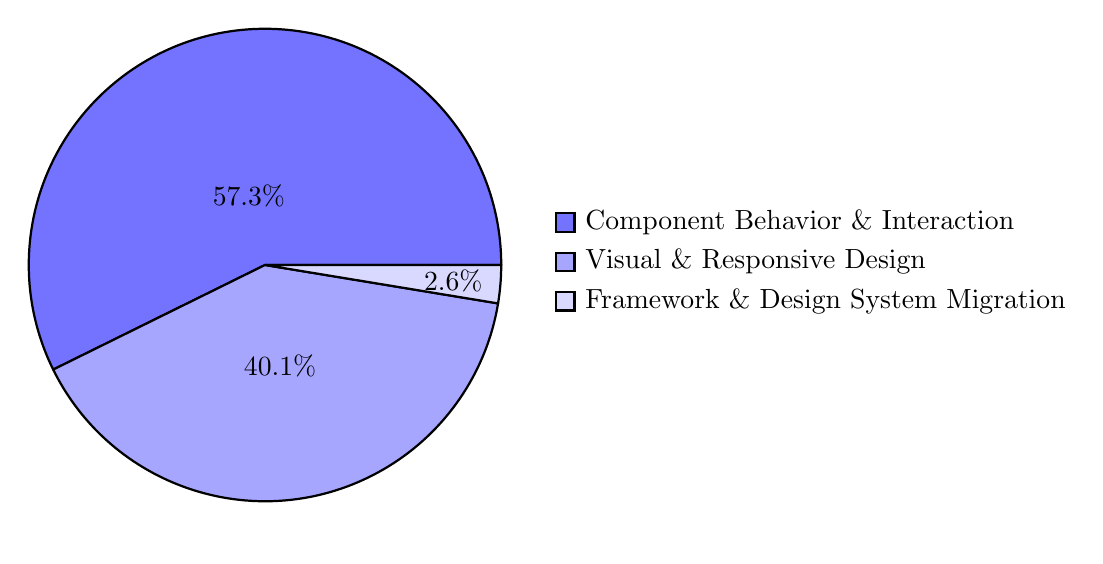
\begin{tikzpicture}
\pie[radius=3, text=legend,
     color={blue!55, blue!35, blue!15}]{
57.3/Component Behavior \& Interaction,
40.1/Visual \& Responsive Design,
2.6/Framework \& Design System Migration
}
\end{tikzpicture}
\caption{Distribution of Modernization \emph{Aspects} across all
UI-related commits in the mined pool (LLM-classified).}
\label{fig:aspects-full}
\end{figure}

\begin{figure}[htbp]
\centering
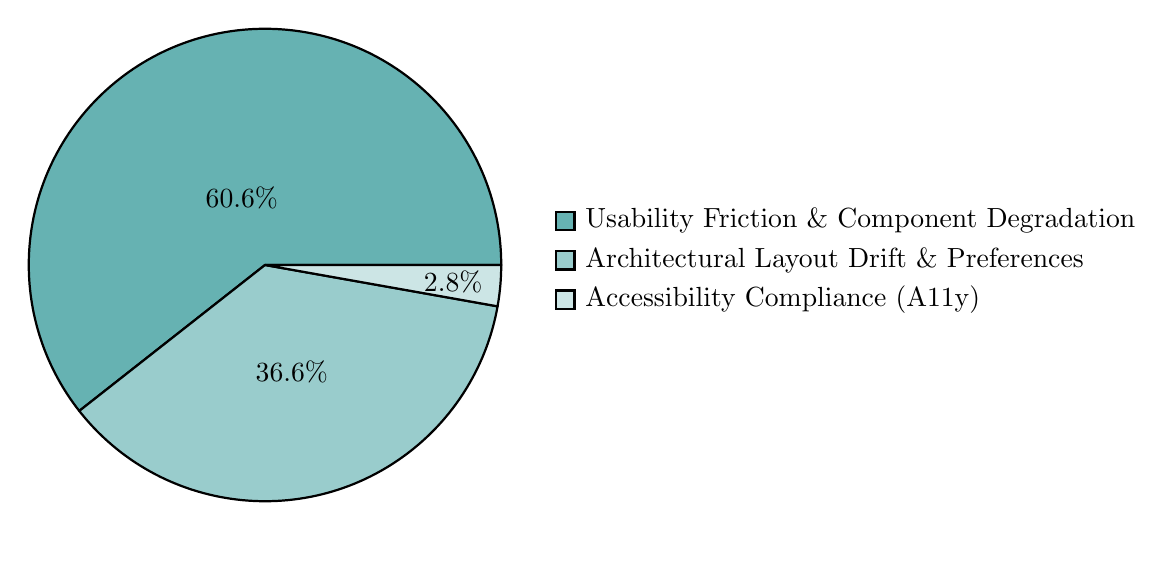
\begin{tikzpicture}
\pie[radius=3, text=legend,
     color={teal!60, teal!40, teal!20}]{
60.6/Usability Friction \& Component Degradation,
36.6/Architectural Layout Drift \& Preferences,
2.8/Accessibility Compliance (A11y)
}
\end{tikzpicture}
\caption{Distribution of Modernization \emph{Causes} across all
UI-related commits in the mined pool (LLM-classified).}
\label{fig:causes-full}
\end{figure}

\paragraph{How each commit was assigned an Aspect and a Cause.}
Each UI-related commit was assigned exactly one \emph{Aspect} (\emph{what}
changed in the interface) and one \emph{Cause} (\emph{why} the change was
made), inferred from the commit message together with the repository
context. The \emph{Aspect} captures the structural nature of the change and
maps one-to-one onto the modernization spectrum
(Section~\ref{sec:spectrum}). A commit was labelled \textbf{Component
Behavior and Interaction} (Up-Level) when it altered how a component reacts
to input or state (e.g., hover, focus, or disabled feedback, animations
and transitions, navigation, pagination or scrolling, input handling, or the
repair of a broken, frozen, or flickering interaction). It was labelled
\textbf{Visual and Responsive Design} (Intermediate-Level) when it changed
only the appearance of existing components without altering their behavior (color, spacing, typography, theming, light/dark mode, alignment, icons,
or responsive breakpoints). It was labelled \textbf{Framework and Design
System Migration} (Down-Level) when it adopted, replaced, or upgraded a UI
library or design system, introduced or propagated design tokens, or moved
components onto a shared component library.

The \emph{Cause} captures the human-centric trigger behind the change,
following the three categories of Section~\ref{sec:method}. A commit was
assigned \textbf{Accessibility Compliance} when it explicitly targeted an
accessibility barrier --- Accessible Rich Internet Applications (ARIA) attributes, colour-contrast, screen-reader
support, keyboard operability, or touch-target sizing. It was assigned
\textbf{Architectural Layout Drift and Preferences} when it re-aligned
elements to a design guideline, repositioned or reconfigured interface
elements, adjusted spacing or theme configuration, or added a user
preference or toggle. It was assigned \textbf{Usability Friction and
Component Degradation} when it removed visual clutter or resolved an
operational defect degrading the experience (flicker, overflow, a stuck
loader, a rendering glitch, or a frozen interaction). When a commit carried
signals for more than one category (for instance, a dark-mode contrast fix
that is both an accessibility and a visual change), the \emph{dominant}
change described in the message, the primary problem the commit set out
to solve, determined the label, so that every commit contributes to a
single Aspect and a single Cause and the two distributions are directly
comparable.

\paragraph{Reconciling the LLM Aspect distribution with the spectrum-tier
distribution.}
The Aspect proportions in Figure~\ref{fig:aspects-full} (57.3\% Component
Behavior, 40.1\% Visual and Responsive Design, 2.6\% Framework and Design
System Migration) differ substantially from the spectrum-tier proportions
in Table~\ref{tab:phase3_tiers} and Figure~\ref{fig:spectrum_pie}
(35--36\% Up-Level, 32.5--32.9\% Intermediate-Level, 28.5--31.1\%
Down-Level), even though each Aspect maps one-to-one onto a tier
(Section~\ref{sec:aspects}). The two figures measure different things and
are not expected to coincide. The spectrum-tier distribution is produced by
unsupervised K-Means over TF-IDF vectors and by the manual tier labels that
follow the same operational rule (Table~\ref{tab:operationalization}): a
commit is counted as Down-Level whenever it touches \texttt{package.json} or
global stylesheet configuration, regardless of whether the message states an
explicit migration intent. Because Down-Level commits are captured
predominantly through the file-type condition rather than a UI keyword
(Table~\ref{tab:cluster_empirical_results}, keyword-match rate 16.4\%), this
tier absorbs a large volume of routine dependency and configuration edits.
The LLM Aspect classifier instead assigns \emph{Framework and Design System
Migration} only when the message describes an actual library adoption,
replacement, upgrade, or design-token propagation, and attributes the
remaining dependency- and build-level edits to the component-behavior or
visual change they accompany. The LLM distribution should therefore be read
as an intent-based estimate of \emph{deliberate} modernization work and is
the basis for our answer to RQ1, whereas the K-Means tier volumes serve only
as an internal check that the three tiers are lexically separable (ANOVA
$F = 7{,}022.63$, $p < 0.000001$).

\paragraph{Accessibility as the least frequent cause.}
Although we list Accessibility Compliance first among the modernization
causes (Section~\ref{sec:method}), following its prominence in the
human-centric issue taxonomy of Khalajzadeh et
al.~\cite{khalajzadeh2022how}, it is the rarest trigger in our corpus
(2.8\%, Figure~\ref{fig:causes-full}). Two factors plausibly contribute.
First, accessibility work is frequently folded into a broader visual or
behavioral change and is then labelled by its dominant intent rather than
as a standalone accessibility fix. Second, explicit accessibility commits
often use narrow, standards-oriented vocabulary (\texttt{aria},
\texttt{role}, \texttt{contrast}, \texttt{focus-visible}) that the Phase~2
keyword condition covers only partially, so many accessibility commits
enter the pool through the file-type condition and are then classified by
their surface change. The low share is therefore best read as a lower bound
on accessibility-motivated modernization rather than as evidence that OSS
projects seldom address accessibility.


%% ================================================================
\newpage
\section{Conclusion}
%% ================================================================

In this study, we addressed the gap between general OSS usability research
and the specific question of how and why open-source interfaces are
modernized. Prior work has shown that OSS contributors tend to hold a
system-centric rather than user-centric view of their projects
\cite{wang2022how, andreasen2006usability}, that usability and UX
discussions in OSS issue trackers are shaped largely by personal opinion
rather than systematic process \cite{cheng2018how}, that human-centric
issues raised on GitHub can be reliably categorized
\cite{khalajzadeh2022how}, and that design system communities concentrate
their discussions on three structurally distinct concerns (component
behavior, visual design, and framework migration)
\cite{lamine2022understanding}. However, none of this prior work connects
a specific human-centric cause to the concrete UI change it produced
within a single study.

We addressed this gap with RQ0, RQ1, and RQ2. For RQ0, we found that
\textbf{56.5\%} of all recent commit activity in actively maintained
JavaScript/TypeScript OSS repositories corresponds to UI-design or
usability modernization, establishing the scale of front-end evolution
work before classifying its kind or trigger. We then proposed a
two-dimensional classification scheme adapted from these prior
taxonomies, that separates modernization \emph{causes} (Accessibility
Compliance Overhauls, Architectural Layout Drift and Preferences,
Usability Friction and Component Degradation) from modernization
\emph{aspects} (Component Behavior and Interaction Refactoring, Visual
and Responsive Design Adjustment, Framework and Design System
Migration), and a three-tier spectrum (Down-, Intermediate-, and
Up-Level) that measures how deep a given modernization effort reaches
into the codebase. Because each Aspect category maps one-to-one onto a
spectrum level, RQ1 can be operationalized directly as a classification
task.

Our multi-condition mining pipeline, combining word-boundary keyword
matching, file-type detection, a date boundary, and commit-level prefix
exclusion, achieves a filter precision of $\approx$96\% over a
200-commit manual validation sample, corroborated by an LLM-assisted
double-check yielding the same $\approx$96\% precision on the stratified
$\approx$1,000-commit sample. Applied to our corpus of 25,061 Phase~2
commits across 346 actively maintained OSS repositories, the pipeline
yields an estimated 24,059 ($\pm$877) genuinely UI-related commits
available for Cause/Aspect classification.

Future work should apply the full Cause/Aspect classification to the
retained commit pool and statistically verify that the three spectrum
tiers correspond to meaningfully different intensities of UI
modernization across a larger and more diverse set of OSS projects.
Future work should also examine whether specific causes (e.g.,
accessibility) are systematically associated with specific aspects
(e.g., framework migration), which would give OSS maintainers a more
predictive understanding of how a given human-centric issue is likely
to be resolved.

\newpage
\section*{Acknowledgments}

This research was conducted by Eliz Payaslı as part of a
research internship in the Software Engineering \& Technology (SET) group
of the Department of Mathematics and Computer Science at Eindhoven
University of Technology (TU/e). The work is supervised by Jacob Krüger
and Alexander Nolte.

% ==========================================
% BIBLIOGRAPHY
% ==========================================
\begin{thebibliography}{99}

%% ── Core SE/HCI references ──────────────────────────────────────────────────

\bibitem{wang2022how}
W. Wang, J. Cheng, and J. L. C. Guo,
``How Do Open Source Software Contributors Perceive and Address Usability?''
\textit{IEEE Software}, vol.~39, no.~1, pp.~76--83, 2022.

\bibitem{hellman2022characterizing}
J. Hellman, J. Chen, M. S. Uddin, J. Cheng, and J. L. C. Guo,
``Characterizing User Behaviors in Open-Source Software User Forums:
An Empirical Study,''
in \textit{Proc.\ CHASE}, pp.~46--55, 2022.

\bibitem{cheng2018how}
J. Cheng and J. L. C. Guo,
``How Do the Open Source Communities Address Usability and UX Issues?
An Exploratory Study,''
in \textit{Extended Abstracts CHI}, pp.~1--6, 2018.

\bibitem{lamine2022understanding}
Y. Lamine and J. Cheng,
``Understanding and Supporting the Design Systems Practice,''
\textit{arXiv preprint arXiv:2205.10713}, 2022.

\bibitem{khalajzadeh2022how}
H. Khalajzadeh, M. Shahin, H. O. Obie, and J. Grundy,
``How are Diverse End-user Human-centric Issues Discussed on GitHub?''
in \textit{Proc.\ ICSE SEIS}, pp.~1--11, 2022.

\bibitem{khalajzadeh2025towards}
H. Khalajzadeh et al.,
``Towards Integrated Dashboards for Better Management of Human-centric Issues,''
\textit{Automated Software Engineering}, vol.~32, pp.~115--128, 2025.

\bibitem{llerena2019adapting}
L. Llerena, N. Rodriguez, J. W. Castro, and S. T. Acu\~{n}a,
``Adapting Usability Techniques for Application in Open Source Software,''
\textit{Information and Software Technology}, vol.~107, pp.~48--64, 2019.

\bibitem{castro2025how}
J. W. Castro et al.,
``How to Improve Usability in OSS Projects?''
\textit{Informatics}, vol.~12, no.~1, pp.~45--58, 2025.

\bibitem{raza2012users}
A. Raza, L. F. Capretz, and F. Ahmed,
``Users' Perception of Open Source Usability: An Empirical Study,''
\textit{Engineering with Computers}, vol.~28, no.~2, pp.~109--121, 2012.

\bibitem{andreasen2006usability}
M. S. Andreasen, H. V. Nielsen, S. O. Schr{\o}der, and J. Stage,
``Usability in Open Source Software Development: Opinions and Practice,''
\textit{Information Technology and Control}, vol.~35, no.~3A,
pp.~303--312, 2006.

%% ── MSR methodology ──────────────────────────────────────────────────────────

\bibitem{kalliamvakou2014promises}
E. Kalliamvakou et al.,
``The Promises and Perils of Mining GitHub,''
in \textit{Proc.\ MSR}, ACM, pp.~92--101, 2014.

\bibitem{silva2016refactor}
D. Silva, N. Tsantalis, and M. T. Valente,
``Why We Refactor? Confessions of GitHub Contributors,''
in \textit{Proc.\ FSE}, ACM, pp.~858--870, 2016.

\bibitem{vidoni2022systematic}
M. Vidoni,
``A Systematic Process for Mining Software Repositories: Results from a
Systematic Literature Review,''
\textit{Information and Software Technology}, vol.~144, p.~106791, 2022.
\url{https://doi.org/10.1016/j.infsof.2021.106791}

\bibitem{logemann2024file}
M. Logemann,
``Analyzing File Structure Evolution of Software Projects,''
Master's Thesis, TU/e, 2024.
\url{https://pure.tue.nl/ws/portalfiles/portal/351955771/Logemann_M.pdf}

\bibitem{herzig2013}
K. Herzig, S. Just, and A. Zeller,
``It's Not a Bug, It's a Feature: How Misclassification Impacts Bug Prediction,''
in \textit{Proc.\ ICSE}, pp.~392--401, 2013.

\bibitem{levin2017}
S. Levin and A. Yehudai,
``Boosting Automatic Commit Classification into Maintenance Activities
by Utilizing Source Code Changes,''
in \textit{Proc.\ SOFTENG}, pp.~14--19, 2017.

\bibitem{github2024}
GitHub,
``GitHub REST API Documentation,''
2024.
\url{https://docs.github.com/en/rest}

%% ── Statistics and ML ────────────────────────────────────────────────────────

\bibitem{cohen1960}
J. Cohen,
``A Coefficient of Agreement for Nominal Scales,''
\textit{Educational and Psychological Measurement}, vol.~20, no.~1,
pp.~37--46, 1960.

\bibitem{salton1988}
G. Salton and C. Buckley,
``Term-Weighting Approaches in Automatic Text Retrieval,''
\textit{Information Processing \& Management}, vol.~24, no.~5,
pp.~513--523, 1988.

\bibitem{macqueen1967}
J. B. MacQueen,
``Some Methods for Classification and Analysis of Multivariate Observations,''
in \textit{Proc.\ 5th Berkeley Symposium on Mathematical Statistics and
Probability}, vol.~1, pp.~281--297, 1967.

\bibitem{hou2024}
X. Hou et al.,
``Large Language Models for Software Engineering: A Systematic Literature Review,''
\textit{IEEE Transactions on Software Engineering}, vol.~50, no.~9,
pp.~2366--2395, 2024.

%% ── Initial sample repositories ──────────────────────────────────────────────

\bibitem{appsmith}
Appsmith, \textit{appsmithorg/appsmith}, GitHub.
\url{https://github.com/appsmithorg/appsmith}

\bibitem{drawio}
jgraph, \textit{jgraph/drawio}, GitHub.
\url{https://github.com/jgraph/drawio}

\bibitem{plane}
makeplane, \textit{makeplane/plane}, GitHub.
\url{https://github.com/makeplane/plane}

\bibitem{chatwoot}
Chatwoot, \textit{chatwoot/chatwoot}, GitHub.
\url{https://github.com/chatwoot/chatwoot}

\bibitem{outline}
Outline, \textit{outline/outline}, GitHub.
\url{https://github.com/outline/outline}

\bibitem{freecodecamp}
freeCodeCamp, \textit{freeCodeCamp/freeCodeCamp}, GitHub.
\url{https://github.com/freeCodeCamp/freeCodeCamp}

\bibitem{calcom}
Cal.com, \textit{calcom/cal.com}, GitHub.
\url{https://github.com/calcom/cal.com}

\bibitem{commit:grafana:a11y}
{Grafana Labs},
``Accessibility: Link Operation label to dropdown,''
GitHub commit \texttt{c24f6c7}, 2026.
\url{https://github.com/grafana/grafana/commit/c24f6c70c4318e8f764ca75aa11865e51de549a0}

\bibitem{commit:clashverge:freeze}
{clash-verge-rev contributors},
``fix: throttle WebSocket subscriptions to prevent UI freeze,''
GitHub commit \texttt{824bcc7}, 2026.
\url{https://github.com/clash-verge-rev/clash-verge-rev/commit/824bcc77eb5d33af5756193f85209dcf9f2a8d54}

\bibitem{commit:gitlens:wip}
{GitKraken},
``Persists WIP commit drafts in the graph panel,''
GitHub commit \texttt{4ed4eb1}, 2026.
\url{https://github.com/gitkraken/vscode-gitlens/commit/4ed4eb1c00673ca8f0e8096cc11f81367e8fb989}

\bibitem{commit:portainer:invisible}
{Portainer},
``fix(ui): display invisible special characters in web editor,''
GitHub commit \texttt{c4cc9cf}, 2026.
\url{https://github.com/portainer/portainer/commit/c4cc9cf1c74aaa4f11cf5c8ef724306061d62751}

\bibitem{commit:redisinsight:accordion}
{Redis},
``Insights panel fixes -- text overflow, tooltip text, and accordion layout,''
GitHub commit \texttt{c71ca66}, 2026.
\url{https://github.com/redis/RedisInsight/commit/c71ca66ff836256b80a1662130025a5b045c2a72}

\bibitem{commit:labelstudio:toast}
{HumanSignal},
``fix: Toast does not auto-dismiss and persists across page navigation,''
GitHub commit \texttt{3f0b1c7}, 2026.
\url{https://github.com/HumanSignal/label-studio/commit/3f0b1c79ded0dfc378819e3d892dddff9f40baca}

\bibitem{commit:mattermost:menu}
{Mattermost},
``Pass through menu props to popout menu item, guard at menu definition,''
GitHub commit \texttt{2fb38fe}, 2026.
\url{https://github.com/mattermost/mattermost/commit/2fb38fe71d7b5d34885dd7d38915c0ff929048e1}

\bibitem{commit:angular:contrast}
{Google},
``fix(docs-infra): readable contrast for DEV/EXP api badges in light mode,''
GitHub commit \texttt{0010ad5}, 2026.
\url{https://github.com/angular/angular/commit/0010ad5910186540fd85e980bff7d608613c738e}

\bibitem{commit:dyad:hover}
{dyad-sh},
``fix Project hover visibility,''
GitHub commit \texttt{8aa893b}, 2026.
\url{https://github.com/dyad-sh/dyad/commit/8aa893b1ba20baa525f0cdbf3bd17cbd4620d37e}

\bibitem{commit:aionui:sider}
{iOfficeAI},
``style(sider): lighten section title rest color and unify top margin,''
GitHub commit \texttt{7856e63}, 2026.
\url{https://github.com/iOfficeAI/AionUi/commit/7856e63c50a7c88b56d3205817e0359470b388be}

\bibitem{commit:mattermost:darkmode}
{Mattermost},
``Fix Data Spillage reviewer pill background in dark mode,''
GitHub commit \texttt{7d1ee48}, 2026.
\url{https://github.com/mattermost/mattermost/commit/7d1ee48c080bb0a2d47ee0e6ddffaa75ec7d12c9}

\bibitem{commit:jitsi:avatar}
{Jitsi},
``fix(mobile) clamp computed avatar sizes to positive values,''
GitHub commit \texttt{d6d0209}, 2026.
\url{https://github.com/jitsi/jitsi-meet/commit/d6d0209decc0571fdd9937671fc59d2d8247fe0d}

\bibitem{commit:aionui:button}
{iOfficeAI},
``style(sider): always show team create button,''
GitHub commit \texttt{f2b90b0}, 2026.
\url{https://github.com/iOfficeAI/AionUi/commit/f2b90b03eb16f059d906c3010f7b9c439b4a1bf6}

\bibitem{commit:signoz:checkbox}
{SigNoz},
``refactor: replace antd Checkbox with @signozhq/ui Checkbox,''
GitHub commit \texttt{31e4012}, 2026.
\url{https://github.com/SigNoz/signoz/commit/31e4012fe59aadd3c382e9f5727543c0857452cf}

\bibitem{commit:labelstudio:tokens}
{HumanSignal},
``feat: Adjusts design-tokens converter to properly parse font-families,''
GitHub commit \texttt{f80a362}, 2026.
\url{https://github.com/HumanSignal/label-studio/commit/f80a362a763f5047306fdafd9496d61889590eac}

\bibitem{commit:metamask:designsystem}
{MetaMask},
``chore: upgrade design system packages v41.0.0,''
GitHub commit \texttt{42f1b96}, 2026.
\url{https://github.com/MetaMask/metamask-extension/commit/42f1b965caf3308048fa35b098b48eefc3d95144}

\bibitem{commit:portainer:tailwind}
{Portainer},
``chore(tailwind): format tailwind class order,''
GitHub commit \texttt{ab3e095}, 2026.
\url{https://github.com/portainer/portainer/commit/ab3e0956a43b97f1cd1f8b8b25bdb20e9866c1b9}

\bibitem{commit:superset:antdesign}
{Apache},
``chore(deps): bump @ant-design/icons,''
GitHub commit \texttt{44777cc}, 2026.
\url{https://github.com/apache/superset/commit/44777cc110930cf7ac15e3ac0211ef1bdc49fe73}

\bibitem{commit:mattermost:react}
{Mattermost},
``Add user setting to experimentally enable concurrent React rendering mode,''
GitHub commit \texttt{8c8f28f}, 2026.
\url{https://github.com/mattermost/mattermost/commit/8c8f28f943e811572e16c63f9dfd80b4e3fe081a}

\end{thebibliography}

\end{document}